% !TeX spellcheck = en_US
% !TeX document-id = {cf032f19-4427-4a50-b0ba-ddee651fb980}
% !TeX program = txs:///pdf-chain
% TeX program = txs:///dvi-chain
%DVI -> PS -> PDF
% 10.1016/j.compstruc.2017.04.006 
% OJO VERIFICAR IDIOMA GB

%\documentclass[preprint,12pt,authoryear,letterpaper,times]{elsarticle}
%\documentclass[final,1p,times,twocolumn,authoryear]{elsarticle}
\documentclass[12pt,letterpaper]{article}

\usepackage{parskip} 
\usepackage[margin=3cm]{geometry}
%\usepackage{times}
\usepackage{braket}
\usepackage{mathtools} \mathtoolsset{showonlyrefs} %show only referenced equations
%\usepackage[latin1]{inputenc}
\usepackage[utf8]{inputenc}
%\usepackage[T1]{fontenc}
\usepackage{psfrag}
\usepackage[spanish]{babel}
\usepackage{mathrsfs}  % mathscr
\usepackage{bbm} % R Q N Z symbols
\usepackage{url}
\usepackage{natbib}
\usepackage{amsmath,amssymb,amsthm,amsfonts}

% FOR USE WITH THE TODONOTES PACKAGE:
%\usepackage[table,xcdraw]{xcolor}
\usepackage{xcolor}
\usepackage[spanish,textwidth=2cm]{todonotes} %todonotes goes after xcolor (messages, what to do!)
\newcommand\todoin[2][]{\todo[inline, caption={2do}, #1]{\begin{minipage}{\textwidth-4pt}#2\end{minipage}}}

\newcommand{\pf}{P_\text{\textnormal{f}}}
\newcommand{\LP}{\underline{P_{\Gamma}}}
\newcommand{\UP}{\overline{P_{\Gamma}}}
\newcommand{\rv}[1]{{\uppercase{#1}}}    %random variable
\newcommand{\ve}[1]{{\boldsymbol{#1}}}
\newcommand{\ma}[1]{{\boldsymbol{#1}}}
\newcommand{\dd}{\operatorname{d} \!}
%\newcommand{\nuevo}[1]{\textsf{\textcolor{red}{#1}}}
\newcommand{\nuevo}[1]{#1}
\def\bigtimes{\mathbin{\vcenter{\hbox{\Large $\times$}}}} %\mbox{\Large$\times$} = \bigtimes
%\newcommand{\nuevo}[1]{{#1}}

\newtheorem{thm}{Theorem}
\newtheorem{cor}{Corollary}

\usepackage[colorlinks=true,citecolor=blue,%
plainpages=false,pdfpagelabels,%
breaklinks]{hyperref}
\hypersetup{pdffitwindow=false}

\usepackage{hypernat} % in this way [sort&compress]{natbib} and hyperref will work together

\usepackage{breakurl}

\usepackage{graphicx}

\title{Deducción de la ecuación $\ma{q}^{(e)} = \ma{K}^{(e)} \ve{a}^{(e)} - \ma{f}^{(e)}$ para el EF de barra de dos nodos}
\date{}
\begin{document}
    \maketitle

\begin{figure}[ht]
    \centering
    \makebox[\textwidth][c]{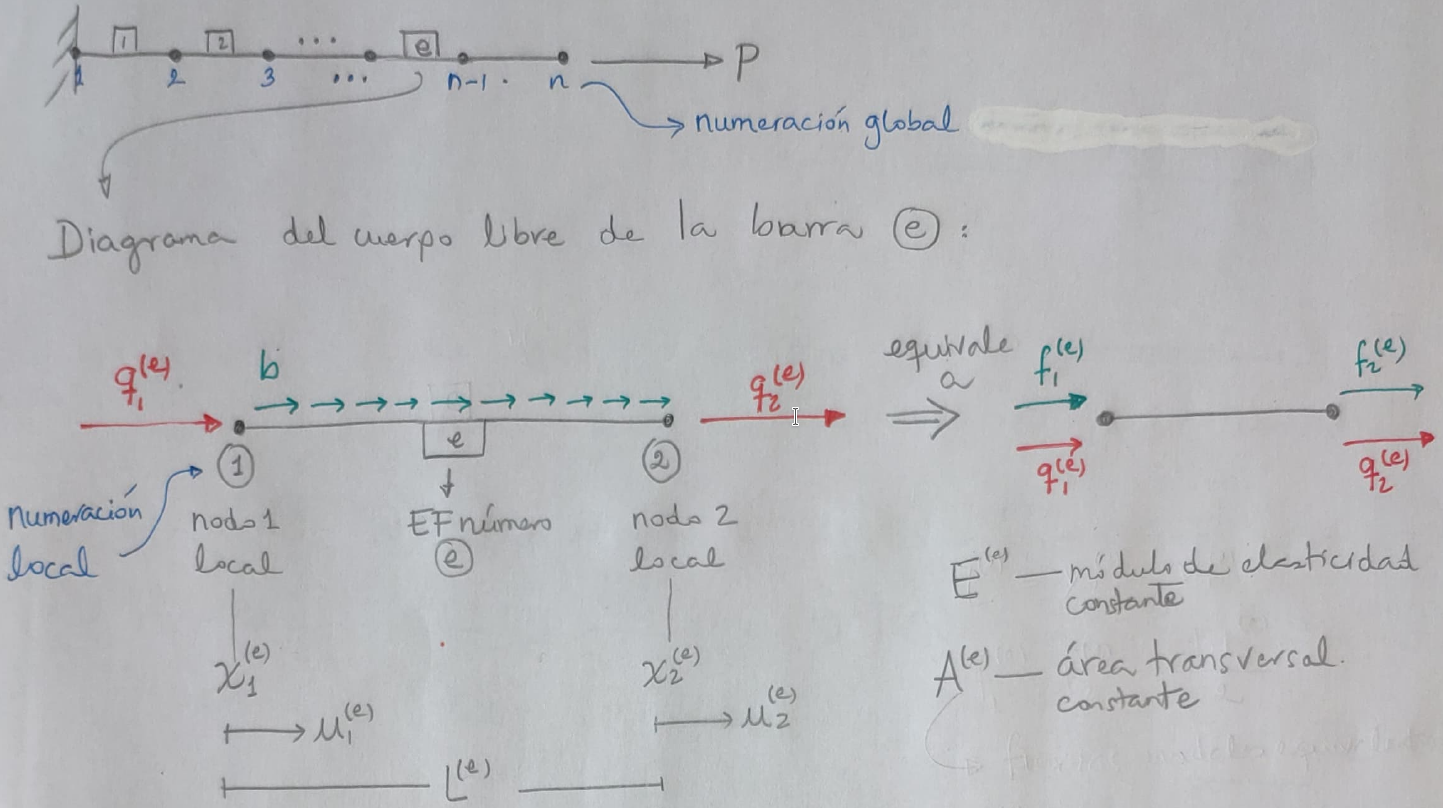
\includegraphics[width=1.2\textwidth]{fig}}
%    \includegraphics[width=0.7\textwidth]{EF_barra_2_nodos}
%    \includegraphics[width=\textwidth]{../codigo/1D/EF_barra_2_nodos.pdf}

\vspace{0.5cm}

\begin{tabular}{ll}
    $u_1^{(e)}$, $u_2^{(e)}$                        & desplazamientos nodales       \\
    $x_1^{(e)}$, $x_2^{(e)}$                        & coordenadas globales          \\
    $L^{(e)}=x_2^{(e)} - x_1^{(e)}$                 & longitud de la barra          \\
    $f_1^{(e)}=f_2^{(e)}=\frac{b^{(e)} L^{(e)}}{2}$ & fuerzas nodales equivalentes  \\
    $q_1^{(e)}$, $q_2^{(e)}$                        & fuerzas nodales de equilibrio \\
    $A^{(e)}$                                       & área transversal constante    \\
    $E^{(e)}$                                       & módulo de elasticidad constante
\end{tabular}

    \caption{Diagrama de cuerpo libre de la barra $e$}
    \label{eq:fuerzas_sobre_EF}
\end{figure}



\section{Cálculo de la deformación longitudinal}
\begin{equation}
\varepsilon_x = \frac{\Delta L^{(e)}}{L^{(e)}} = \frac{u_2^{(e)} - u_1^{(e)}}{L^{(e)}}
\end{equation}

\section{Cálculo de los esfuerzos normales}
Para relacionar los esfuerzos y las deformaciones se utiliza la ley de Hooke en 1D:
\[
\sigma_x^{(e)} = E^{(e)} \varepsilon_x^{(e)} = E^{(e)} \frac{u_2^{(e)} - u_1^{(e)}}{L^{(e)}} 
\]

\section{Cálculo de la fuerza axial}

\[f_{ax}^{(e)}=A^{(e)} \sigma_x^{(e)} = \underbrace{\frac{E^{(e)} A^{(e)}}{L^{(e)}}}_{k^{(e)}} \left [ u_2^{(e)}-u_1^{(e)} \right ]\]

Aquí el término $k^{(e)} = \frac{E^{(e)} A^{(e)}}{L^{(e)}}$ se conoce como la \emph{rigidez axial de la barra}.

\section{Equilibrio de fuerzas}
Consideremos una barra sometida a una tracción de intensidad $F$:
\[
F \leftarrow\rule[0.5mm]{1cm}{0.1cm}\rightarrow F
\]
Para esta barra se tiene que:

Lado izquierdo (nodo 1):
\begin{align}
    \left( f_1^{(e)} + q_1^{(e)} \right) &= -F = -f_{ax}^{(e)} = k^{(e)} \left[u_1^{(e)} - u_2^{(e)} \right] 
    &\implies\quad
q_1^{(e)} &= k^{(e)} u_1^{(e)} - k^{(e)} u_2^{(e)} - f_1^{(e)} \label{eq:1}
\end{align}

Lado derecho (nodo 2):
\begin{align}
\left ( f_2^{(e)} + q_2^{(e)} \right ) &= +F = +f_{ax}^{(e)} = k^{(e)} \left[u_2^{(e)} - u_1^{(e)} \right] 
&\implies\quad
q_2^{(e)} = -k^{(e)} u_1^{(e)} + k^{(e)} u_2^{(e)} - f_2^{(e)} \label{eq:2}
\end{align}

De las ecuaciones~\eqref{eq:1} y~\eqref{eq:2} se obtiene la llamada \emph{ecuación de equilibrilio para la barra}:
\begin{equation}
\underbrace{%
\begin{bmatrix}
	q_1^{(e)} \\
	q_2^{(e)}
\end{bmatrix}}_{\ve{q}^{(e)}}
=
\underbrace{\begin{bmatrix}
	+k^{(e)} & -k^{(e)}\vphantom{q_1^{(e)}}\\
	-k^{(e)} & +k^{(e)}\vphantom{q_2^{(e)}}
\end{bmatrix}}_{\ma{K}^{(e)}}
\underbrace{\begin{bmatrix}
	u_1^{(e)}\\
	u_2^{(e)}
\end{bmatrix}}_{\ve{a}^{(e)}}
-
\underbrace{\begin{bmatrix}
	f_1^{(e)}\\
	f_2^{(e)}
\end{bmatrix}}_{\ve{f}^{(e)}}.
\end{equation}

\begin{tabular}{p{0.7cm} p{14cm}}
	$\ve{q}^{(e)}$ & vector de fuerzas nodales de equilibrio (reacciones) de la barra $e$ \\
	$\ma{K}^{(e)}$ & matriz de rigidez de la barra $e$; esta es función únicamente de la geometría de la barra ($A^{(e)}$ y $L^{(e)}$) y de sus propiedades mecánicas ($E^{(e)}$) \\
	$\ve{a}^{(e)}$ & vector de desplazamientos nodales de la barra $e$ \\
	$\ve{f}^{(e)}$ & vector de fuerzas nodales equivalentes de la barra $e$
\end{tabular}

\section{Ejemplo}
iguales para todas las barras

Diagramas de cuerpo libre de las barras y de los nodos

las fuerzas nodales equivalentes se trasladan a los nodos

\subsection{Ecuación de equilibrio para cada barra}
La ecuación de equilibrio para cada barra es
\begin{equation}
\begin{bmatrix}
	q_1^{(e)}\\ 
	q_2^{(e)}
\end{bmatrix}
=
\begin{bmatrix}
	k^{(e)} & -k^{(e)}\\ 
	-k^{(e)} &  k^{(e)}
\end{bmatrix}
\begin{bmatrix}
	u_1^{(e)}\\ 
	u_2^{(e)}
\end{bmatrix}
-
\begin{bmatrix}
	f_1^{(e)}\\ 
	f_2^{(e)}
\end{bmatrix}
\end{equation}
donde $e = 1,\ 2,\ 3$ y 
\begin{equation}
k^{(1)}=k^{(2)}=\frac{EA}{L} \qquad \qquad k^{(3)}=\frac{EA}{\frac{L}{2}}=\frac{2EA}{L}.
\end{equation}

\subsection{Ecuación de equilibrio para cada nodo}

Hacemos la compatibilidad entre los desplazamientos y fuerzas locales y globales en cada nodo

\begin{table}[h]
	\centering
	\begin{tabular}{c|c|c|}
		\cline{2-3}
		& {\color[HTML]{3166FF} 1} & {\color[HTML]{3166FF} 2} \\ \hline
		ulticolumn{1}{|c|}{{\color[HTML]{3166FF} 1}} & 1                        & 3                        \\ \hline
		ulticolumn{1}{|c|}{{\color[HTML]{3166FF} 2}} & 2                        & 3                        \\ \hline
		ulticolumn{1}{|c|}{{\color[HTML]{3166FF} 3}} & 3                        & 4                        \\ \hline
	\end{tabular}
	\caption{Matriz LaG(e, nodo local)}
	\label{tab:LaG}
\end{table}

\begin{align}
R_1= k^{(1)} u_1 - k^{(1)} u_3 - \frac{bL}{2}\\
R_2= k^{(2)} u_2 - k^{(2)} u_3 - \frac{bL}{2}\\
0  =- k^{(1)} u_1 + k^{(1)} u_3 - k^{(2)} u_2 + k^{(2)} u_3 + k^{(3)} u_3 - k^{(3)} u_4 - \left( \frac{P}{2} + \frac{bL}{2} + \frac{bL}{2} \right)\\
0  =- k^{(3)} u_3 + k^{(3)} u_4 - P
\end{align}


\[
\underbrace{\begin{bmatrix}
		R_1\\ 
		R_2\\ 
		0\\ 
		0
\end{bmatrix}}_{ \mathbf{q}}
=
\underbrace{\begin{bmatrix*}[r]
		k^{(1)} & 0 & -k^{(1)} & 0\\ 
		0 & k^{(2)} & -k^{(2)} & 0\\ 
		-k^{(1)} & -k^{(2)} &  k^{(1)}+k^{(2)}+k^{(3)} & -k^{(1)}\\ 
		0 & 0 & -k^{(3)} & k^{(3)}
\end{bmatrix*}}_{ \mathbf{K}}
\underbrace{\begin{bmatrix}
		u_1\\ 
		u_2\\ 
		u_3\\ 
		u_4
\end{bmatrix}}_{ \mathbf{a} }
-
\underbrace{\begin{bmatrix}
		\frac{bL}{2}\\ 
		\frac{bL}{2}\\ 
		\frac{P}{2} + bL\\ 
		P
\end{bmatrix}}_{ \mathbf{f} }
\]

el ensamblaje de este sistema de ecuaciones se fundamenta en que en cada nodo la suma de las fuerzas externas e internas \(q_i^{(e)}\) debe ser igual.

\begin{tabular}{ll}
	$\mathbf{q}$ & vector de fuerzas nodales de equilibrio global (\textit{reaction matrix}) \\
	$\mathbf{K}$ & matriz de rigidez global (\textit{stiffness matrix}) \\
	$\mathbf{a}$ & vector de desplazamientos nodales global (\textit{displacement matrix}) \\
	$\mathbf{f}$ & vector de fuerzas nodales equivalentes global (\textit{load matrix}) \\
\end{tabular}

La ecuación de equilibrio \(\mathbf{q}= \mathbf{Ka}-\mathbf{f}\) de una estructura compuesta de barras se obtiene a partir de la regla sencilla que expresa que en cada nodo la suma de las fuerzas nodales de equilibrio \(q_i^{(e)}\) debidas a las diferentes barras que concurren en dicho nodo es igual a la sumatoria de fuerzas exteriores que actúan en dicho nodo, esto es:

\begin{equation}
	\substack{\text{En el nodo}\\ \text{j-ésimo}} \sum_{e \epsilon E_j} q_{\text{GaL}(e,j)}^{(e)} = \sum_i R_j^{\text{exterior}(i)}
\end{equation}

donde \(E_j\) son el conjunto de todas las barras que concurren en el nodo de numeración global \(j\)

Observe que cada fila de \(\mathbf{q}= \mathbf{Ka}-\mathbf{f}\) corresponde a una ecuación * desarrollada para un grado de libertad

El proceso de obtención de \(\mathbf{q}= \mathbf{Ka}-\mathbf{f}\) recibe el nombre de ensamblaje matricial.

La solución de \(\mathbf{q}= \mathbf{Ka}-\mathbf{f}\) proporciona los valores de los desplazamientos y las reacciones en todos los nodos de la estructura

\begin{table}[h]
	\centering
	\begin{tabular}{c|c|c|c|c|}
		\cline{2-5}
		& {\color[HTML]{3166FF} 1} & {\color[HTML]{3166FF} 2} & {\color[HTML]{3166FF} 3} & {\color[HTML]{3166FF} 4} \\ \hline
		ulticolumn{1}{|c|}{{\color[HTML]{3166FF} 1}} & 1 & X & 2 & X \\ \hline
		ulticolumn{1}{|c|}{{\color[HTML]{3166FF} 2}} & X & 1 & 2 & X \\ \hline
		ulticolumn{1}{|c|}{{\color[HTML]{3166FF} 3}} & X & X & 1 & 2 \\ \hline
	\end{tabular}
	\caption{Matriz GaL(e, número global)}
	\label{tab:GaL}
\end{table}

El ensamblaje matricial puede realizarse también de la siguiente forma:

\[
\mathbf{K} = \underbrace{\begin{bmatrix}
		x & \cdot & x & \cdot\\ 
		\cdot & \cdot & \cdot & \cdot\\ 
		x & \cdot & x & \cdot\\ 
		\cdot & \cdot & \cdot & \cdot
\end{bmatrix}}_{\mathbf{K^{(1)}}}
+
\underbrace{\begin{bmatrix}
		\cdot & \cdot & \cdot & \cdot\\ 
		\cdot & x & x & \cdot\\ 
		\cdot & x & x & \cdot\\ 
		\cdot & \cdot & \cdot & \cdot
\end{bmatrix}}_{\mathbf{K^{(2)}}}
+
\underbrace{\begin{bmatrix}
		\cdot & \cdot & \cdot & \cdot\\ 
		\cdot & \cdot & \cdot & \cdot\\ 
		\cdot & \cdot & x & x\\ 
		\cdot & \cdot & x & x
\end{bmatrix}}_{\mathbf{K^{(3)}}}
\]

\[
\mathbf{f} = \underbrace{\begin{bmatrix}
		\frac{bL}{2}\\ 
		0\\ 
		\frac{bL}{2}\\ 
		0
\end{bmatrix}}_{(1)}
+
\underbrace{\begin{bmatrix}
		0\\
		\frac{bL}{2}\\ 
		\frac{bL}{2}\\ 
		0
\end{bmatrix}}_{(2)}
+
\underbrace{\begin{bmatrix}
		0\\
		0\\ 
		0\\ 
		0
\end{bmatrix}}_{(3)}
+
\underbrace{\begin{bmatrix}
		0\\
		0\\ 
		\frac{P}{2}\\ 
		P
\end{bmatrix}}_{\substack{\text{cargas}\\ \text{puntuales}}}
\]

Finalmente, se calculan las fuerzas axiales

\[f_{ax}^{(e)} = k^{(e)} \left ( u_2^{(e)} - u_1^{(e)} \right ) \qquad e=1,2,3\]
	
\end{document}